\documentclass[conference]{IEEEtran}
\IEEEoverridecommandlockouts

\usepackage[utf8]{inputenc}
\usepackage[ngerman]{babel}
\usepackage{cite}
\usepackage{graphicx}
\usepackage{textcomp}
\usepackage{tabularx}

\begin{document}
\title{Sicherheitsrisiken und Schutzmechanismen in IoT-Anwendungen}
    \author{
      \IEEEauthorblockN{1\textsuperscript{st} Florian Hansen} \\
      \textit{Hochschule Flensburg}\\
      Flensburg, Germany \\
      florian-hansen@stud.hs-flensburg.de
    }
  \maketitle

  % Insert sections here using \input{sections/section.tex}
  \section{Einleitung}
\textit{Internet of Things (kz. IoT)} bezeichnet die Vernetzung von Geräten  über das Internet.
Diese werden oftmals, aufgrund der Verbindung zum Internet, auch als \textit{"intelligente Geräte" 
(engl. smart devices)} bezeichnet. Die Endgeräte können dabei sehr unterschiedlich sein, so reichen
diese von von einfachen Messgeräten bis hinzu komplexen medizinischen Implataten. \\

Aufgrund der Anbindung der Geräte an das Internet, ist die Kommunikationen mit diesen 
einfacher und Daten können leichter extrahiert und übermittelt werden. Diese Prozesse
können zudem automatisiert werden, wodurch keine weitere menschliche Interaktion
benötigt wird und Zeit bzw. Kosten eingespart werden können. Dadurch ist nicht verwunderlich,
dass die Anzahl an IoT-Geräten in den letzten Jahren stark zugenommen hat. So sollen bis Ende
2020 über 25 Milliarden Geräte über das Internet vernetzt sein.\\

Die beeindruckende Anzahl an IoT-Geräten zeigt, dass die Technologie sich heutzutage etabliert hat,
doch sollten hierbei nicht die Sicherheitsrisiken bei der Verwendung von IoT-Geräten außer acht
gelassen werden. Abhängig vom Anwendungsbereich der Geräte können diese für essentielle 
Funtkionalitäten eines System zuständig sein oder mit sehr sensiblen Daten arbeiten. 
Geräte, welche nicht ausreichend geschützt sind, können durch Angriffe bspw.  heruntergefahren
werden, was in Abhängigkeit zum Anwendungsbereich zu erheblichen Schäden führen kann. \\

Im Rahmen diese Ausarbeitung werden die Anwendungsbereiche, Sicherheitsrisiken und Schutzmechanismen
von IoT-Geräten vorgestellt und anhand eines praktischen Beispieles demonstriert.


  




  \section{IoT Anwendungsbereiche}
Aufgrund der allgemeinen Digitalisierung vieler Abläufe und Branchen werden IoT-Geräte umfangreich eingesetzt,
in dem folgenden Kapitel sollen einige Anwendungsbereiche der IoT vorgestellt werden. 

\subsection{Umweltbeobachtung}
Bei der Umweltbeobachtung werden bestimmte Bereiche der Umwelt auf bestimmte ökologische Parameter überwacht. 
So werden bspw. die Luft-, Wasser- oder Bodenqualität von bestimmten Gebieten oder Standorten 
untersucht, um potentielle Umweltprobleme oder -gefahren frühzeitig feststellen zu können. \\

Ein detailliertes Beispiel wäre die Erdbebenüberwachung, bei der IoT-Geräte mit seismischen Sensoren
ausgestattet werden, um frühzeitig Erdbeben zu erkennen. Im Falle eines Erdbebens können die Geräte
weitere System benachrichtigen, welche daraufhin Versorgungseinrichtungen oder  Datenzentren
abschalten, sowie Menschen in kritischen Wohngebieten benachrichtigen können.

\subsection{Gesundheitswesen}
Ärzte benötigen oftmals stetige Information zum körperlichen Zustand eines Patienten, vor allem um
herauszufinden, ob eine bestimmte Behandlung zum gewünschten Erfolg führt. IoT-Geräte, im speziellen
kleine medizinische Implantate, können Ärzte dabei unterstützen bestimmte Gesundheitswerte auszulesen und 
zu versenden bzw. selbständig auszuwerten. Ärzte können dadurch, ohne das physische auftreten der Patienten,
Untersuchungen und Diagnosen durchführen, was sowohl dem Arzt und Patient Zeit und Aufwand einsparen kann.

\subsection{Industrie}
In der Produktion von Gütern finden IoT-Geräte sehr unterschiedliche Verwendungszwecke. Mithilfe der IoT können
bspw. gesamte Lieferketten optimiert werden, indem IoT-Geräte bestimmte Teilprozesse (Produktion, Transport, etc.)
überwachen und in bestimmten Situation zielgerichtete Maßnahmen einleiten. Außerdem werden mithilfe von IoT-Geräten eine 
Vielzahl von Daten ausgehoben, welche in wachsenden Anwendungsbereichen wie Big Data Analysen oder Künstlicher Intelligenz 
benötigt werden.

\subsection{Wearables}
Bei Wearables handelt es sich um technische Geräte, welche direkt am Körper getragen werden und mit verschiedenen 
Sensoren ausgestattet sind. Die bekanntesten Beispiele für Wearabeles sind Smartwachtes und Fitnessarmbänder und 
werden für unterschiedliche Anwendungsbereiche wie bspw. Gesundheitswesen, Sport oder Entertainment eingesetzt.


\subsection{Spielzeuge}
IoT-Geräte in Form von Spielzeugen sind oftsmals mit Lautsprecher, Mikrofonen und wieteren Komponenten ausgesattet
und mit dem Internet verbinden. Funktionalitäten, welche klassische Spielzeuge nicht haben, wäre bspw. eine integrierte
Spracherkennung, bei dir die Aussagen der Kinder aufgenommen, über ein weiteres System ausgewertet und das Spielzeug
demensprechend reagiert. Aufgrund der Verbindung zum Internet stehen den Spielzeugen eine Vielzahl von neuen Möglichkeiten
zur Verfügung.
  \section{Angriffsmöglichkeiten}\label{sec:possible-attacks}
Wie in fast jedem anderen System müssen vor allem IoT-Anwendungen besonders
bezüglich ihrer Sicherheit betrachtet werden. Die Anwendungsentwicklung
innerhalb des IoT ist geprägt von vielseitig komplexen Problemen beim Etablieren
der IT-Sicherheit. Grundsätzlich können Sicherheitsrisiken in drei Bereichen
auftreten, die hier kurz erläutert werden sollen \cite{paper}.

\subsection{Herausforderungen bei mobilen Geräten}
\paragraph{Heterogenität}
Dieser Bereich behandelt Probleme, die durch die Vielzahl an
Anwendungsmöglichkeiten in dem IoT entstehen. Dazu zählen unter anderem
die verbauten Hardware-Komponenten, Protokolle für die Kommunikation unter
Geräten und Variationen zwischen Geräten und ihrer Rechenleistung \cite{paper}.

\paragraph{Ressourcenbeschränkung}
Nicht jedes Gerät beinhaltet einen leistungsstarken Rechner. Oft stößt man bei
der Entwicklung von IoT-Geräten auf das Problem, dass nicht genug Speicher oder
Rechenleistung vorhanden ist. Nicht nur bei der Implementation der eigentlichen
Anwendung macht dies Probleme. Bereits etablierte Sicherheitsalgorithmen können
aufgrund fehlender Leistung nicht verwendet werden, da sie sich als
unpraktikabel in dem IoT herausstellen. Sicherheitsziele können also aufgrund
nicht ausreichender Hardware nicht erreicht werden \cite{paper}. Ein Beispiel
hierfür ist das Arbeiten mit einer Cloud. Sicherheitsziele sind hier unter
anderem die Privatsphäre des Benutzers. Die üblichen kryptographischen
Algorithmen, z.B. die attribut-basierte Verschlüsselungen und Pairings, stellen
sich als sehr unpraktikabel heraus, da diese zu viel Rechenleistung für die
Berechnungen von bilinearen Abbildungen benötigen. Eine vielversprechende Lösung
ist das Auslagern rechenintensiver Schritte an einen leistungsstarken Server
\cite{phoabe}.

\paragraph{Dynamische Netzwerktopologie}
Gerade bei mobilen Geräten innerhalb des IoT haben wir mit ``losen'' Verbindungen
zu tun. Zum Beispiel ist es möglich, dass ein Smartphone mit diversen
WLAN-Hotspots interagiert und damit keine feste Position innerhalb eines
Netzwerkes besitzt \cite{paper}.

\subsection{Definition von Sicherheit}\label{sec:def-security}
Damit die Sicherheit trotz der oben erwähnten Herausforderungen ge\-währ\-lei\-stet
werden kann, genügt es nicht, dass allseits bekannte CIA-Dreieck zu betrachten.
Laut \cite{paper} sind Vertraulichkeit, Integrität und Verfügbarkeit nicht die
einzigen Voraussetzungen, um Sicherheit für IoT-Geräte zu definieren.
Stattdessen müssen individuelle Anforderungen für jeden Anwendungsbereich
definiert werden.

Komplexe Anlagen besitzen zum Beispiel verschiedenste Sensoren und Aktoren, um
beispielsweise Verfahrenstechniken anzuwenden und diese zu über\-wachen. Diese
Sensoren werden häufig beim Implementieren von IT-Sich\-er\-heit vernachlässigt,
nachdem sie verbaut wurden. Mögliche Sicherheitsanforderungen für
diesen Bereich sind Vertraulichkeit, Authentifizierung,
Nachrichtenauthentizität, Integrität, Verfügbarkeit, Zuverlässigkeit, Frische
der Daten und Fälschungsdetektierung \cite{paper}.

Andere Bereiche des IoT benötigen jedoch andere Anforderungen an die
IT-Sicherheit. Im Gesundheitswesen wird die Privatsphäre des Patienten eine
größere Rolle spielen, als bei technischen Anlagen, sodass die Anforderungen
abweichen. Diese sind hier unter anderem Verfügbarkeit, Zuverlässigkeit,
Authentifizierung, Integrität, Vertraulichkeit, Privatsphäre,
Nachrichtenauthentizität, Fälschungsdetektierung, Verantwortlichkeit und
Nichabstreitbarkeit \cite{paper}.

\subsection{Sicherheitsrisiken pro Domäne}
Im vorherigen Abschnitt wurde auf verschiedene IoT-Domänen und ihren
Sicherheitsanforderungen eingegangen. Kurz zusammengefasst ist jede Domäne
unterschiedlich zu behandeln, wenn es um Sicherheit geht. Angreifer, die
Schwachstellen in solchen Systemen finden, haben unter Umständen Zugriff auf
eine große Menge von sensiblen Daten. Mögliche Angriffe können auf Grundlage der
Sicherheitsanforderungen aus Abschnitt \ref{sec:def-security} abgeleitet werden
\cite{paper} und werden in Tabelle \ref{tab:security-threats} dargestellt.

\begin{table*}[t]
  \centering
  \label{tab:security-threats}
  \begin{tabularx}{\textwidth}{lX}
    \textbf{Anwendungsdomäne} & \textbf{Mögliche Angriffe}\\
    \hline
    Umgebungsüberwachung & DoS/DDoS, MitM, Node capture, Sinkhole, Hello flood,
    Traffic analysis, Hacking, Side channel, Sybil, Selective forwarding, Back
    hole, Tampering, Wormhole, Masquerading \\

    Gesundheitswesen & DoS/DDoS, MitM, Malicious code, Spoofing, Hacking,
    Tampering, Eavesdropping, Hijacking, Replay, Backdoof, Tag tracking, Tag
    cloning, Identity theft, Masquerading, Node capture, Side channel \\

    Feuerwehr & DoS/DDoS, MitM, Sybil, Hello flood, Node capture, Sinkhole,
    Black hole, Selective forwarding, Hacking, Tampering, Malicious code,
    Hijacking, Side channel, Traffic analysis, GPS jamming \\

    Herstellung & DoS/DDoS, MitM, Masquerading, Backdoor, Identity theft,
    Replay, Hijacking, Hacking, Eavesdropping, Selective forwarding, Back hole,
    Sinkhole, Node capture, Sybil, Spoofing, Traffic analysis, Side channel,
    Tampering, Wormhole, Malicious code, Wormhole, Economic espionage \\

    Wearables & DoS/DDoS, Eavesdropping, MitM, Malicious code, Identity theft,
    Hacking, Backdoor, Hijacking, inappropriate network configuration \\

    Spielzeuge & DoS/DDoS, Eavesdropping, MitM, Identity theft, Hijacking,
    Hacking, Backdoor, Masquerading, Spoofing, Malicious code, inappropriate
    network configuration
  \end{tabularx}
  \caption{Sicherheitsrisiken pro Domäne \cite{paper}}
\end{table*}

  \section{Verteidigung gegen Angriffe}\label{sec:defense-against-attacks}

\paragraph{Gegenmaßnahmen für unsichere Web-Interfaces und Netzwerkdienste.}
Damit ein Fluten von Authentifizierungsanfragen verhindert werden kann, können
Standardports geblockt werden. Für SSH ist dies beispielsweise der Port 22 und
für Telnet der Port 23 bzw. 2323. Grundsätzlich sollten nur die Ports geöffnet
werden, die wirklich benötigt werden. Auch das \textit{Universial Plug and Play
Protocol} (UPnP) sollte deaktiviert werden. Außerdem werden häufig
Standardeinstellungen wie Benutzernamen und Passwörter unverändert übernommen.
Dies ist offensichtlich ein großes Problem, denn ein Angreifer wird diese
Information ohne großen Aufwand herausfinden können. Man sollte also darauf
achten, individuelle und starke Passwörter zu verwenden. Auch die Software
selbst sollte regelmäßig Updates eingespielt bekommen, denn häufig werden
Schwachstellen erst nach einem Release festgestellt und Patches veröffentlicht
\cite{paper}.

\paragraph{Gegenmaßnahmen für Routing-Protokolle.}
Da IoT-Geräte sehr eingeschränkter Natur sind, ist das Schützen von
IoT-Netzwerken eine echte Herausforderung \cite{patel2016}. Sinkhole-Angriffe
können laut \cite{paper} verhindert werden, indem robuste
Authentifikation-Schemata, geografisches Routing und systematisches Rerouting
verwendet werden.  Geografisches Routing bedeutet, dass Datenpakete abhängig der
Position von Knotenpunkten und der Zieladresse innerhalb des Netzwerks
umgeleitet werden.  Die Chancen, dass Forwarding- und Black-Hole-Angriffe
durchführbar sind, können mithilfe von Source-Routing reduziert werden.
Verwendet man Multipath-Routing, dann können Selective-Forwarding-Angriffe
abgewehrt werden. Hierbei werden verschiedene Pfade innerhalb des Netzwerks
verwendet. Hello-Flood-Angriffe können durch bidirektionale Authentifikation
verhindert werden.  Wormhole-Angriffe können ebenfalls durch geografisches
Routing erschwert durchführbar gemacht werden. Aber auch durch physische
Überwachung oder Source-Rou\-ting können Angriffe dieser Art verhindert werden.
Gegenmaßnamen gegen Sybil-Angriffe ist die Evaluierung der Einzigartigkeit von
Geräten im Netzwerk.  Dies bedeutet lediglich, dass jedes Gerät eine eindeutige
Identifikationsnummer besitzen muss. Auch mithilfe von sogenannten
Random-Key-Pre-Dis\-tri\-bu\-tion-Schemata \cite{chan2003} können Sybil-Angriffe
verhindert werden.

\paragraph{Gegenmaßnahmen für Informationstransport.}
Bevor ein Smart-De\-vice einen Datenaustausch beginnt, sollte sich dieses Gerät
vorerst authentifizieren. Ebenfalls sollte eine beidseitige Authentifizierung
implementiert werden, damit beide Parteien verifizieren können, ob es sich um
den richtigen Endpunkt handelt und sie mit dem gewünschten Ziel kommunizieren.
Die Idee hierbei ist, dass zum Beispiel digitale Signaturen (SHA, ECDSA) bzw.
symmetrische äquivalente (HMAC) ausgetauscht werden. Dies dient vor allem für
die Einhaltung der Integrität der Daten. Ebenfalls können Signaturen verwendet
werden, um einen Secure-Boot zu implementieren. Dies hilft dabei, dass das
IoT-Gerät nur Codes ausführt, die vertrauenswürdig, also signiert sind. Vor
allem wird dadurch verhindert, dass zum Beispiel die Firmware des Geräts
überspielt wird. Um die Angriffe abzuwehren, die die Vertraulichkeit betreffen,
werden Informationen über einen sicheren, verschlüsselten Kanal übertragen. Dies
betrifft auch die Kommunikation mit externen Diensten, wie einer Cloud
\cite{paper}.

\paragraph{Gegenmaßnahmen für physische Angriffe.}
Um zum Beispiel Node-Capturing zu verhindern, müssen Geräte physisch versteckt
werden, um den Zugang zu erschweren. Außerdem können die Geräte so gebaut
werden, sodass diese nur sehr schwer auseinanderbaubar sind. USB-Ports sollten
zudem auch geschützt werden, damit ein Angreifer keine Schadsoftware über diese
einspielen kann. Schutzmaßnahmen gegen das Manipulieren von Daten können durch
regelmäßige Änderung der Schlüssel eingeführt werden. Side-Channel-Angriffe
können durch spezielle, resistente Chipsätze verhindert werden.  Das Messen von
elektromagnetische Strahlung muss beim Entwickeln von IoT-Geräten ebenfalls
berücksichtigt werden. Das Verschleiern von Informationen auf diesem Wege muss
also ebenfalls implementiert werden, damit Angreifer nicht mithilfe von
elektrischen Signalen Zugriff bekommen \cite{paper}.

\paragraph{Gegenmaßnahmen für GPS-Jamming.}
Um GPS-Jamming-Angriffe abzuwehren, können Kerbfilter \cite{borio2012}
eingesetzt werden \cite{paper}.

\paragraph{Gegenmaßnahmen für Tag-Tracking und -Cloning.}
Eine Schutzmaßnahme gegen das Tag-Tracking ist, dass die Tags gegenüber einem
Angreifer zufällig aussehen und eine gleiche Verteilung besitzen, damit dieser
keine Schlüsse aus dem Aufbau der Tags ziehen kann. Um Tag-Cloning zu
verhindern, muss sichergestellt werden, dass die eigentlichen Informationen
unter dem Tag nicht zugänglich sind, um einen neuen validen Tag zu erzeugen
\cite{paper}.

\paragraph{Gegenmaßnahmen für falsche Netwerkkonfiguration.}
Die Schutzmaßnahme ist hier sozialer Natur. Ein Schulen der Benutzer über die
Wichtigkeit der IT-Sicherheit ist unabdingbar. Es müssen starke Regeln für
Passwörter verwendet und sicherheitsrelevantes Logging aktiviert werden
\cite{paper}.

  \section{Experiment}
Die Aspekte, welche in \textit{3. Sicherheitsrisiken} und \textit{4. Schutzmechanism} beschrieben wurden, sollen anhand
eines Expirementes verdeutlicht werden. Mithilfe eines selbstgebauten IoT-Gerätes sollen potentielle Sicherheitsrisken, 
welche ein Angreifer ausnutzen kann, sowie Schutzmechanism, um diesen entgegenzuwirken, vorgestellt und erklärt werden.

\subsection{Sicherheitskamera}
Das IoT-Geräte, welches für das Experiment entwickelt werden soll, ist eine Sicherheitskamera, die mithilfe der Kamera
einen Bereich überwacht und dessen Bilderaufnahmen von  weiteren System aufgerufen werden können. \\

Die Sicherheitskamera soll mit einem \textit{Raspberry PI} und einem Kamera-Adapter umgesetzt werden.
Die Bilderaufnahmen, die von der Kamera erstellt werden, sollen über ein Programm ausgelesen und über
einen auf dem \textit{Raspberry PI} laufenden Server abrufbar sein. \\

	\begin{figure}[h]
		\centering
		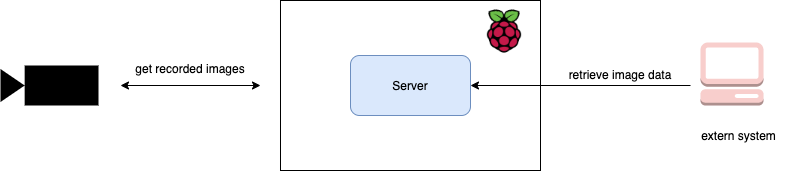
\includegraphics[width=145mm]{images/raspberrypi.png}
		\caption{Sicherheitskamera-Architektur}
		\label{fig:arch-raspberrypi}
	\end{figure}


  \section{Testaufbau}
Bevor wir mit der Durchführung des Experiments beginnen, stellen wir im
Folgenden den Aufbau unserer Testumgebung vor. Da es sich bei \cite{paper} um
ein Framework handelt, welches Entwickler dabei unterstützen soll, neue
IoT-Anwendungen zu entwerfen, müssen wir uns Gedanken über ein mögliches
Szenario machen. Wir haben uns dazu entschieden, eine einfache Sicherheitskamera
zu entwickeln. Hierfür wird im ersten Schritt nach bekannten Frameworks
geschaut, deren Anwendungszweck im IoT-Bereich zu finden ist. Anschließend
sollen diese Frameworks verwendet werden, um die Beispielanwendung umzusetzen.
Dann wird mithilfe des Leitfadens von \cite{paper} untersucht, ob das
entstandene Produkt bezüglich der IT-Sicherheit bestanden hat.

\subsection{Wahl der Komponenten}

Wir haben uns für \textit{aREST} als Framework entschieden, da der Autor dieses
selbst für seinen Online-Dienst verwendet und das Repository auf GitHub unter
allen Projekten, die MQTT als Protokoll verwenden, einen über\-durch\-schnittlichen
Bekanntheitsgrad besitzt. Mithilfe von \textit{aREST} und NodeJS wird eine
Sicherheitskamera entwickelt, die in Echtzeit Bilder übertragen soll. Als
Plattform wird ein Raspberry PI 3B+ mit Raspbian Lite als Betriebssystem und ein
entsprechendes Kameramodul verwendet.

Um zusätzliche Knotenpunkte im Netzwerk zu erzeugen, werden insgesamt zwei
weitere, virtuelle Maschinen (VM) aufgesetzt und mit dem Netzwerk verbunden. Die
erste VM fungiert als MQTT-Broker und versorgt alle Abonnenten mit entsprechenden
Informationen. Geräte, die bestimmte Themen abonnieren, erhalten dementsprechend
eine Nachricht, falls sich der abonnierte Wert verändert. So kann das Netzwerk
theoretisch um weitere Knotenpunkte bzw. Endgeräte erweitert werden und wir
erhalten damit eine realistische Abbildung eines solchen Szenarios. Die zweite
VM stellt den Eindringling bzw. Angreifer des Systems dar und hat später die
Aufgabe, sensible Daten auszuspähen und einzelne Knotenpunkte zu attackieren.
Der gesamte Aufbau wird in Abbildung~\ref{fig:testing-setup} dargestellt.

\begin{figure}
  \centering
  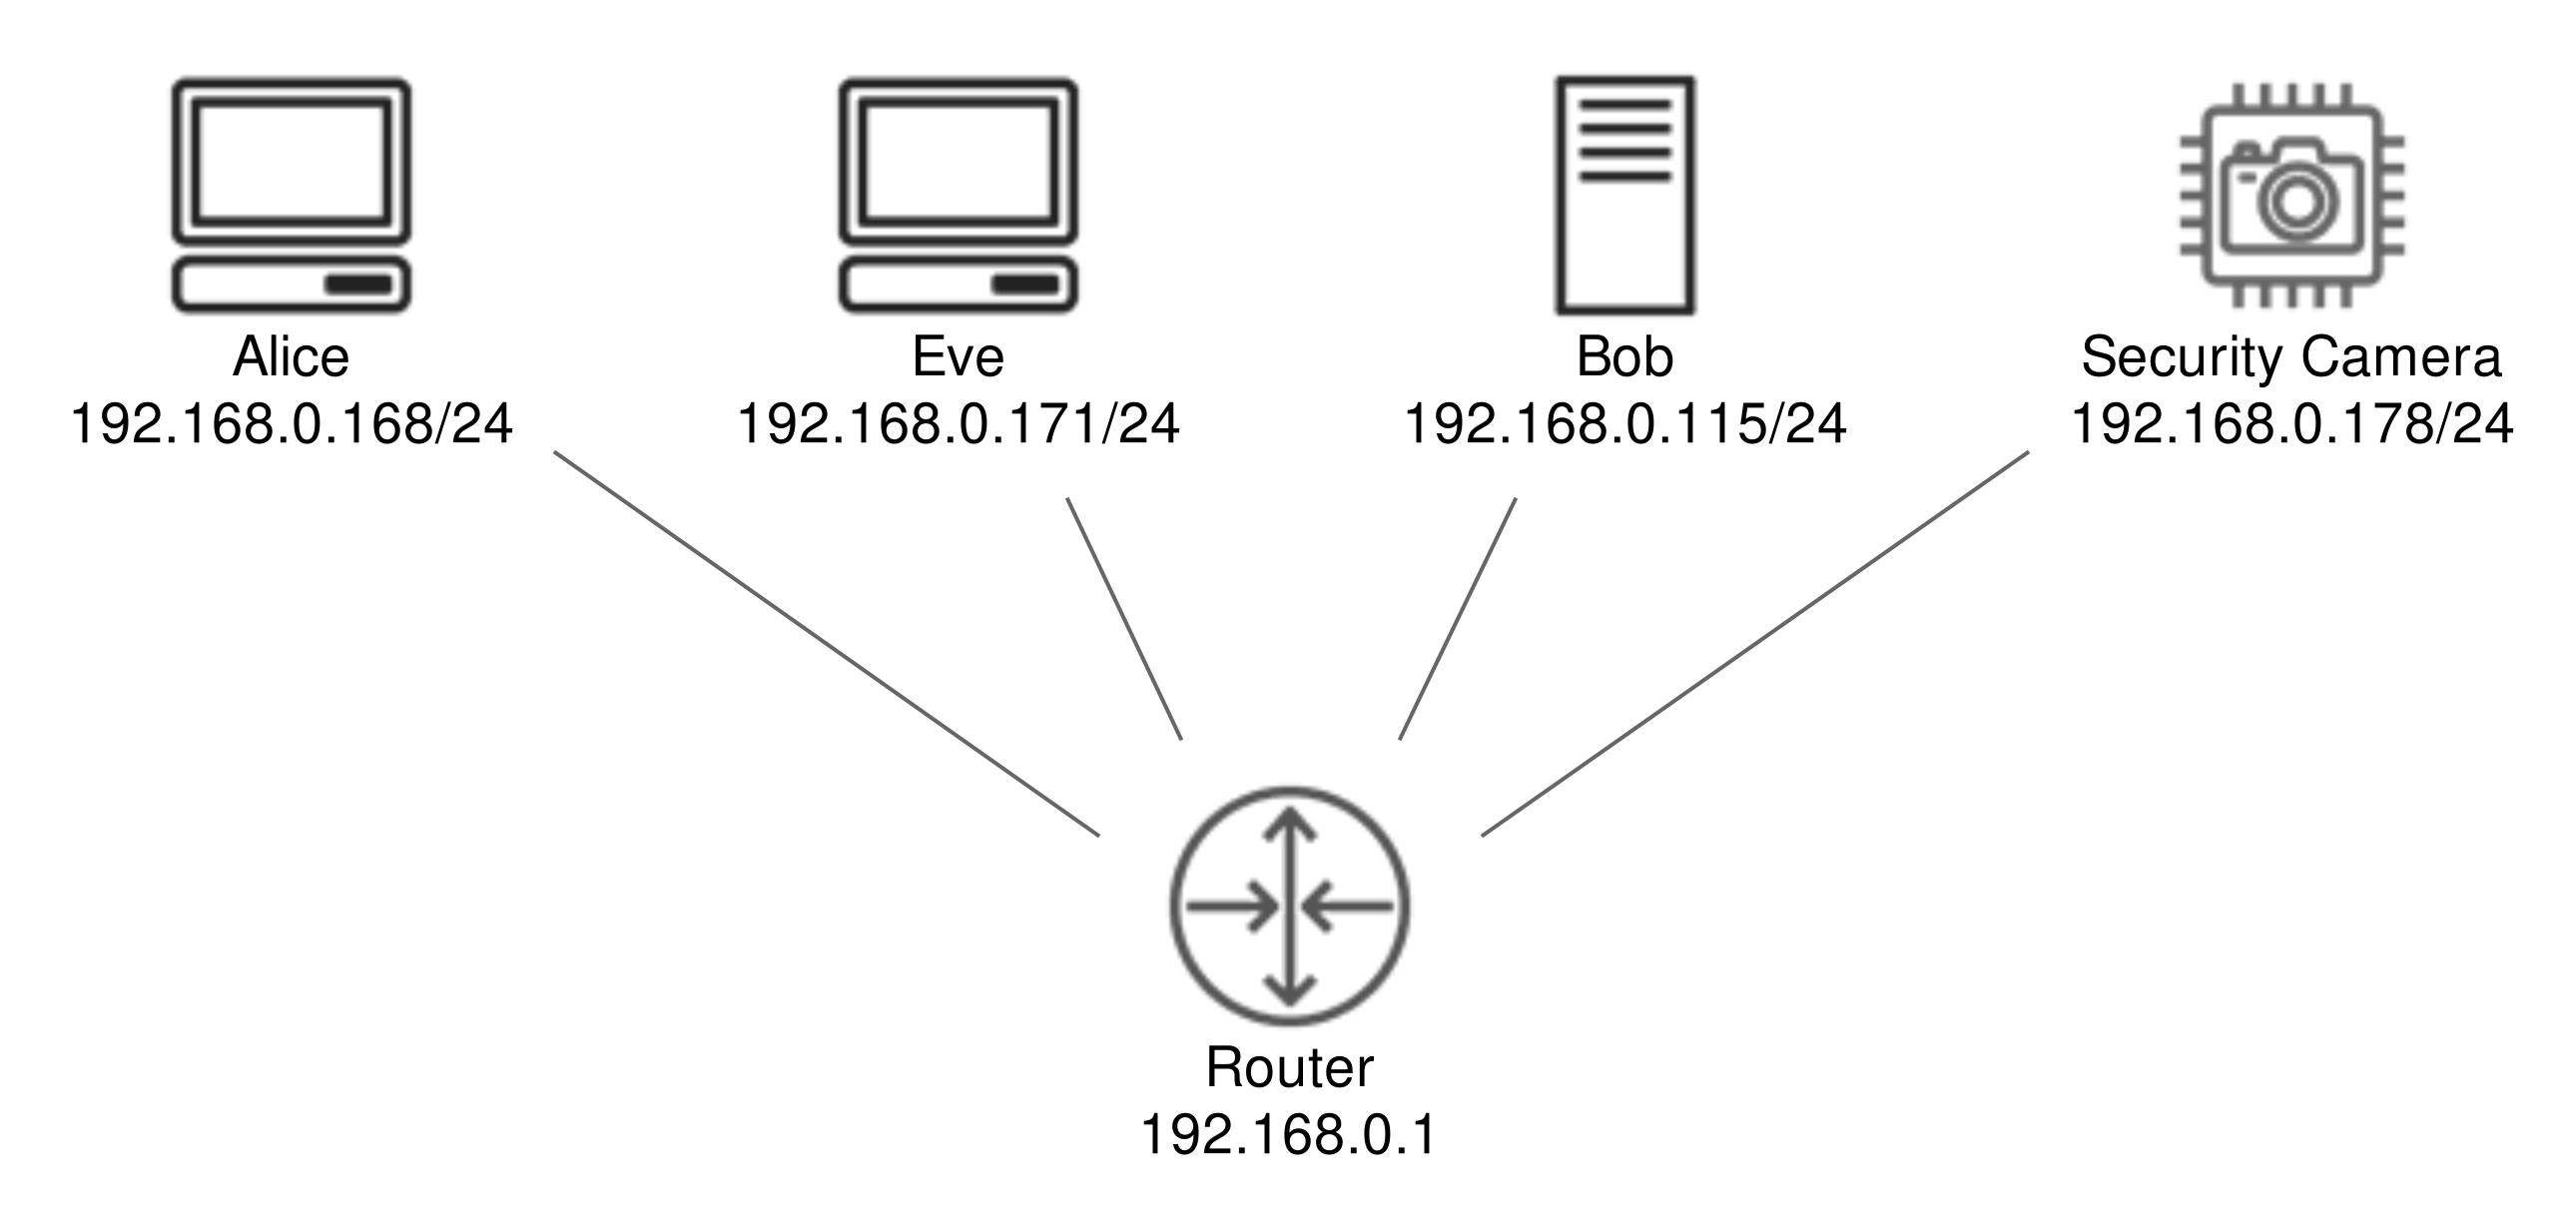
\includegraphics[width=\textwidth]{images/testing-setup}
  \caption{Darstellung des Testaufbaus und dessen Komponenten}
  \label{fig:testing-setup}
\end{figure}

\subsection{Festlegung sensibler Daten}
Damit aussagekräftige Ergebnisse erzielt werden können, muss in erster Linie
festgestellt werden, welche Daten überhaupt sensibel sind. Die Unterscheidung
ist maßgebend für die Analyse der IT-Sicherheit des Systems und hängt immer vom
Kontext der Anwendung ab~\cite{paper}. Zum Beispiel ist es möglicherweise
erwünscht, dass Wetterdaten öffentlich einsehbar sind. Auch wenn diese
von einem Sensor ausgelesen werden, der sich nicht im Besitz des des Anfragenden
befindet. Bei Smart-Home-Systemen ist es jedoch eher selten erwünscht, dass sich
unauthentifizierte Personen Zugang zum Eigenheim beschaffen können. Die
Klassifizierung, ob Daten sensibel sind oder nicht, hängt also vom jeweiligen
Kontext ab. Ein weiteres Beispiel hierfür ist das autonome Fahren. Nicht jeder
sollte sich mit dem eigenen KFZ verbinden und Daten auslesen bzw. Aktoren
bedienen können.

Auch die Sicherheitskamera, die in diesem Experiment entwickelt werden soll,
besitzt aufgrund ihres Einsatzes sensible Daten. Wie üblich sollte nur
authentifiziertes Personal Zugriff zu Aufnahmen der Kamera erhalten. Auch sollte
es nicht einfach möglich sein, die Kamera außer Betrieb zu nehmen. Im Falle
eines Ausfalls könnte der Angreifer bzw. Einbrecher auf das Gelände oder in das
Gebäude eindringen, ohne gesehen zu werden. Zudem sollte es nicht möglich sein,
dass die Aufnahmen der Sicherheitskamera manipuliert bzw. ausgetauscht werden
können. Mögliche Angriffe sind die Manipulation von Daten, die Einschränkung
der Verfügbarkeit, Blackhole-Angriffe bzw. Selective-Forwarding und das Abhören
von Daten (eavesdropping).

  \section{Durchführung des Experiments}
Nachdem der Testaufbau besprochen wurde, gilt es nun in die Rolle des Angreifers
zu schlüpfen und mögliche Angriffe zu diskutieren und auszuführen. Außerdem soll
besprochen werden, wie die Angriffe hätten verhindert werden können, sodass die
Arbeit von~\cite{paper} Anwendung findet. Wie in
Abbildung~\ref{fig:testing-setup} dargestellt, werden die Komponenten zunächst
aufgebaut. Folgende Netzwerkteilnehmer werden konfiguriert:

\begin{itemize}
  \item \textbf{Alice} erhält die IP-Adresse 192.168.2.115 und stellt einen
    MQTT-Client dar. Es werden bestimmte Topics abonniert, sodass dieses Gerät
    benachrichtigt wird, falls sich bestimmte Werte im System ändern.
  \item \textbf{Bob} erhält die IP-Adresse 192.168.2.171 und stellt den
    MQTT-Broker dar. Dieser empfängt Daten von Sensoren und speichert diese
    unter einem bestimmten Topic ab. Abonnenten des Topics werden dann von ihm
    benachrichtigt. Als Anwendung wird \textit{Aedes} verwendet.
  \item Der \textbf{Sicherheitskamera} (Security Camera) wird die IP-Adresse
    192.168.2.178 zugewiesen und dient in dem Aufbau als Sensor. Es werden
    periodisch Bildaufnahmen erzeugt und an Bob, dem Broker, gesendet.
  \item \textbf{Eve} stellt den Angreifer dar und erhält die IP-Adresse
    192.168.2.168.
  \item Der \textbf{Router} stellt mit der IP-Adresse 192.168.2.1 das
    Standard-Gateway des Netzwerks dar.
\end{itemize}

\subsection{Eavesdropping}
Ein entscheidender Grund, warum HTTPS als Ergänzung zu HTTP entwickelt wurde,
ist das Senden und Empfangen von sensiblen Informationen wie Passwörter und
anderen benutzerspezifischen Eigenschaften. Dies ist auch bei MQTT bzw. MQTTS
der Fall. Deshalb wird in diesem Abschnitt untersucht, wie sicher das Framework
\textit{pi-aREST} diesbezüglich ist. Als erster Punkt kann genannt werden, dass
es nicht möglich ist, den Kommunikationsport einzustellen. Dieser ist fest in
das Framework eingearbeitet und lautet 1883, welcher im Allgemeinen als unsicher
gilt. Dieser Port wird meist für das Protokoll MQTT und nicht für das sichere
Äquivalent MQTTS verwendet. Da die Ports jedoch vom Serveradministrator
individuell verwendet werden können, muss nun untersucht werden, ob die
Kommunikation tatsächlich unverschlüsselt verläuft. Hierfür wird auf
\textit{Eve} das Netzwerkanalyse-Tool \textit{Wireshark} installiert und
ausgeführt. Zudem werden die Dienste von der Sicherheitskamera und Bob
gestartet, sodass diese miteinander kommunizieren und Daten kontinuierlich
ausgetauscht werden. Werden Pakete von einem Netzwerkteilnehmer zu einem anderen
gesendet, sind diese an jedem Knotenpunkt im Netzwerk abgreifbar. Jeder
Knotenpunkt entscheidet dann anhand der Paket-Header, ob das jeweilige Paket für
ihn bestimmt ist. Dadurch, dass in der Tat keine Verschlüsselung der Daten
erfolgt, können mithilfe von \textit{Wireshark} Bildaufnahmen ausgespäht werden,
wie Abbildung~\ref{fig:wireshark} zeigt. Gerade für Kameras, dessen Aufnahmen im
Grunde nicht für jedermann zugänglich sein sollen, ist dies eine kritische
Sicherheitslücke. Diese könnte beispielsweise durch ein geeignetes
Verschlüsselungsverfahren geschlossen werden, sodass nur Parteien mit den
jeweiligen geheimen Schlüsseln Zugriff zu den Daten erlangen können. Die
Verwendung des Protokolls MQTTS könnte zum Beispiel die Sicherheitslücke
schließen. Dieses Experiment zeigt, dass durch simples Zuhören sensible Daten
ausgespäht werden können, ohne in den Informationsfluss einzugreifen oder zu
beeinflussen.  Voraussetzung ist natürlich, dass sich der Angreifer im selben
Netzwerk befindet.

\begin{figure}
  \centerline{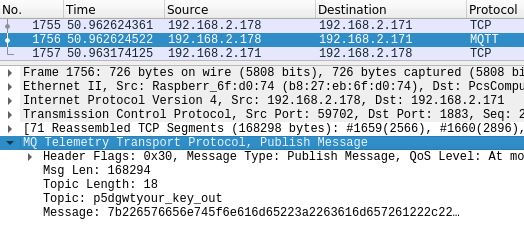
\includegraphics[width=\columnwidth]{images/wireshark}}
  \caption{Ausgespähte Pakete des unsicheren MQTT-Protokolls mit Wireshark}
  \label{fig:wireshark}
\end{figure}

\subsection{Man-in-the-Middle-Angriff}
Bei einem Blackhole-Angriff handelt es sich um einen Denial-of-Service-Angriff
(DoS), bei dem die Verfügbarkeit der Daten angegriffen wird. Dabei wird der
Informationsfluss zwischen zwei Knotenpunkten über eine dritte Instanz
umgeleitet. Anschließend werden bestimmte Informationspakete verworfen, sodass
diese dem eigentlichen Ziel nicht mehr zur Verfügung stehen~\cite{aad2004}. Als
würden die Informationen in ein schwarzes Loch fallen.

Auch dies soll in diesem Experiment exemplarisch durchgeführt werden. Hierfür
werden die Dienste von Bob und der Sicherheitskamera gestartet, sodass ein
Informationsfluss stattfindet. Es werden also wieder kontinuierlich Bilder von
der Kamera aufgenommen und an den Broker gesendet. Das Ziel in diesem Versuch
ist es, die Verbindung zu unterbrechen bzw. Pakete verschwinden zu lassen, ohne
einen kompletten Knotenpunkt des Netzwerks auszuschalten, wie es bei einem
DDoS-Angriff der Fall ist. Die erste Hürde ist also, sich als Angreifer zwischen
die beiden Kommunikationspartner zu schalten, ohne dass diese es bemerken und
anschließend keine Pakete weiterzuleiten. Ein solcher Angreifer wird traditionell
als \textit{Man in the Middle} (MitM) bezeichnet. Es stellt sich nun also die
Frage, wie man den Informationsfluss über eine dritte Instanz leiten kann. Die
einfachste Methode ist das ARP-Spoofing. Hierbei wird den beiden Teilnehmern
vorgetäuscht, man selbst sei der richtige Gesprächspartner.

Das \textit{Address Resolution Protocol} (ARP) ist ein häufig eingesetztes
Protokoll, welches Adressen des \textit{Internet Protocols} (IP) auf Adressen
des \textit{Link-Layers} (MAC-Adressen) abbildet. Teilnehmer des Netzwerks,
welches ARP verwendet, nehmen alle ARP-Pakete an, egal wer diese sendet. Dies
hat vor allem Performancegründe, bildet jedoch eine Schwachstelle für einen
MitM-Angriff im lokalen Netzwerk.

Eve hat nun also die Aufgabe, sich bei Bob als die Sicherheitskamera und bei der
Sicherheitskamera sich als Bob auszugeben. Hierbei wird eine Schwachstelle des
ARP-Protokolls ausgenutzt. ARP implementiert nämlich keine Authentifizierung der
Knotenpunkte, die das Protokoll verwenden. Als Angreifer sendet Eve also
ARP-Pakete, mit denen sie Bob weiß macht, sie sei die Sicherheitskamera. Bob
merkt sich dies und speichert sich den Eintrag in seine persönliche ARP-Tabelle.
Anschließend gibt sich Eve als Bob bei der Sicherheitskamera aus und sendet
entsprechende ARP-Pakete zu ihr. Auch diese merkt sich dies in ihrer eigenen
Tabelle. Hiermit verläuft der Informationsfluss zwischen der Sicherheitskamera
und Bob über Eve. Damit Pakete nun tatsächlich weitergeleitet werden, müsste
dies erst konfiguriert werden. Wird dies nicht getan, werden alle Pakete
einfach zu Eve gesendet und dann verworfen, also genau das, was das
Ziel dieses Versuchs ist. Die Pakete werden somit verschluckt und tauchen nicht
bei dem eigentlichen Zielen auf. Auf das Experiment bezogen bedeutet dies, dass
die aufgenommenen Bilder von der Sicherheitskamera nicht zu dem Broker gelangen
und eine Aktualisierung des entsprechenden Topics ausfällt. Die Verfügbarkeit
wurde damit als grundlegende Sicherheitsanforderung verletzt.

Des Weiteren können nun mächtigere Angriffe durchgeführt werden, wie
beispielsweise das Manipulieren der Bilddaten. Bei einem Einbruch könnte der
Angreifer die Bilder z.B. so verändern, dass dieser nicht auf den Aufnahmen zu
sehen ist. Da das Framework, mit dem die Anwendung entwickelt wurde, lediglich
das MQTT- und nicht das sicherere MQTTS-Protokoll verwendet, kann die Integrität
der Daten nicht gewährleistet werden. Die Verwendung von MQTTS bzw. das
Überprüfen der Integrität könnte dieses Problem also lösen.

  \section{Fazit}
Wir haben besprochen, welche Protokolle in der IoT verwendet werden, um Daten
miteinander kontinuierlich auszutauschen und dass Sicherheitsanforderungen
abhängig von ihrer Domäne sind. So sind Anforderungen an die Automobil-Industrie
andere als die der Spielzeug-Domäne. Eine detaillierte Betrachtung des Kontexts
einer IoT-Anwendung ist demnach essentiell für das Etablieren von IT-Sicherheit.
Mit diesem Wissen haben wir uns ein Projekt bzw. Framework ausgesucht, welches
bekannte Protokolle wie MQTT implementiert und einen Datenaustausch zwischen
IoT-Geräten ermöglicht. Mithilfe dieses Frameworks wurde eine Sicherheitskamera
entwickelt und anschließend auf IT-Sicherheit überprüft. Dabei wurden ebenfalls
die verwendeten Angriffstechniken besprochen. Als Ergebnis kam vor allem heraus,
dass das Framework ausschließlich die Kommunikation über unverschlüsselte Kanäle
anbietet. Dies ist jedoch in sehr vielen IoT-Anwendungen eine Verletzung der
IT-Sicherheit. Besonders bei unserem Beispiel mit der Sicherheitskamera konnten
wir zeigen, dass aufgrund der Tatsache, dass keine geeignete Verschlüsselung
verwendet wird und Bildaufnahmen der Kamera mit einfachsten Mitteln ausgespäht
werden können. Auch schützt das Framework nicht vor Fälschung der Daten, sodass
die Bildaufnahmen manipuliert zum Broker gelangen können.


	\bibliography{literature}
	\bibliographystyle{abbrv}
\end{document}
